% ======================= CHAPTER 3: METHODOLOGY ==========================
\chapter{Methodology}

This chapter describes the dataset, the three architectures, the shared training pipeline, the evaluation metrics, and the proposed decoder. Hyperparameters are stated explicitly so that the experiments can be reproduced.

\section{Dataset: Cholec80}

All experiments use the public Cholec80 dataset~\cite{twinanda2017endonet}: eighty laparoscopic cholecystectomy videos with a phase label and tool-presence labels on every frame. Following the usual protocol~\cite{twinanda2017endonet,jin2018svrcnet,czempiel2020tecno,gao2021transsvnet}, the videos are split by patient into 40 for training (IDs 1--40), 20 for validation (IDs 41--60), and 20 for testing (IDs 61--80). Frames are taken at one per second with OpenCV; the phase labels, originally at 25~fps, are sub-sampled to match. Each frame is resized to $224 \times 224$ pixels and normalised with the ImageNet mean and standard deviation.

During training, the same light augmentations---random horizontal flip, rotation up to $10^\circ$, a random crop with a 10\% margin, and colour jitter---are applied to all frames in a sequence so the sequence stays consistent. Each input sample is eight consecutive frames at one frame per second, giving eight seconds of context.

\begin{table}[H]
\centering
\caption{Phase distribution of the Cholec80 training split (1~fps).}
\label{tab:phase_distribution}
\begin{tabular}{clrr}
\toprule
\textbf{ID} & \textbf{Phase} & \textbf{Frames} & \textbf{Fraction} \\
\midrule
0 & Preparation                & 3,758  & 4.4\% \\
1 & Calot triangle dissection  & 36,886 & 42.7\% \\
2 & Clipping and cutting       & 7,329  & 8.5\% \\
3 & Gallbladder dissection     & 24,119 & 27.9\% \\
4 & Gallbladder packaging      & 3,716  & 4.3\% \\
5 & Cleaning and coagulation   & 7,222  & 8.4\% \\
6 & Gallbladder retraction     & 3,314  & 3.8\% \\
\bottomrule
\end{tabular}
\end{table}

The most common phase (Calot triangle dissection) outnumbers the rarest (Gallbladder retraction) by 11.1 to 1. This is the imbalance the training pipeline is built to handle. Figure~\ref{fig:class_distribution} shows the distribution across the three splits.

\begin{figure}[H]
\centering
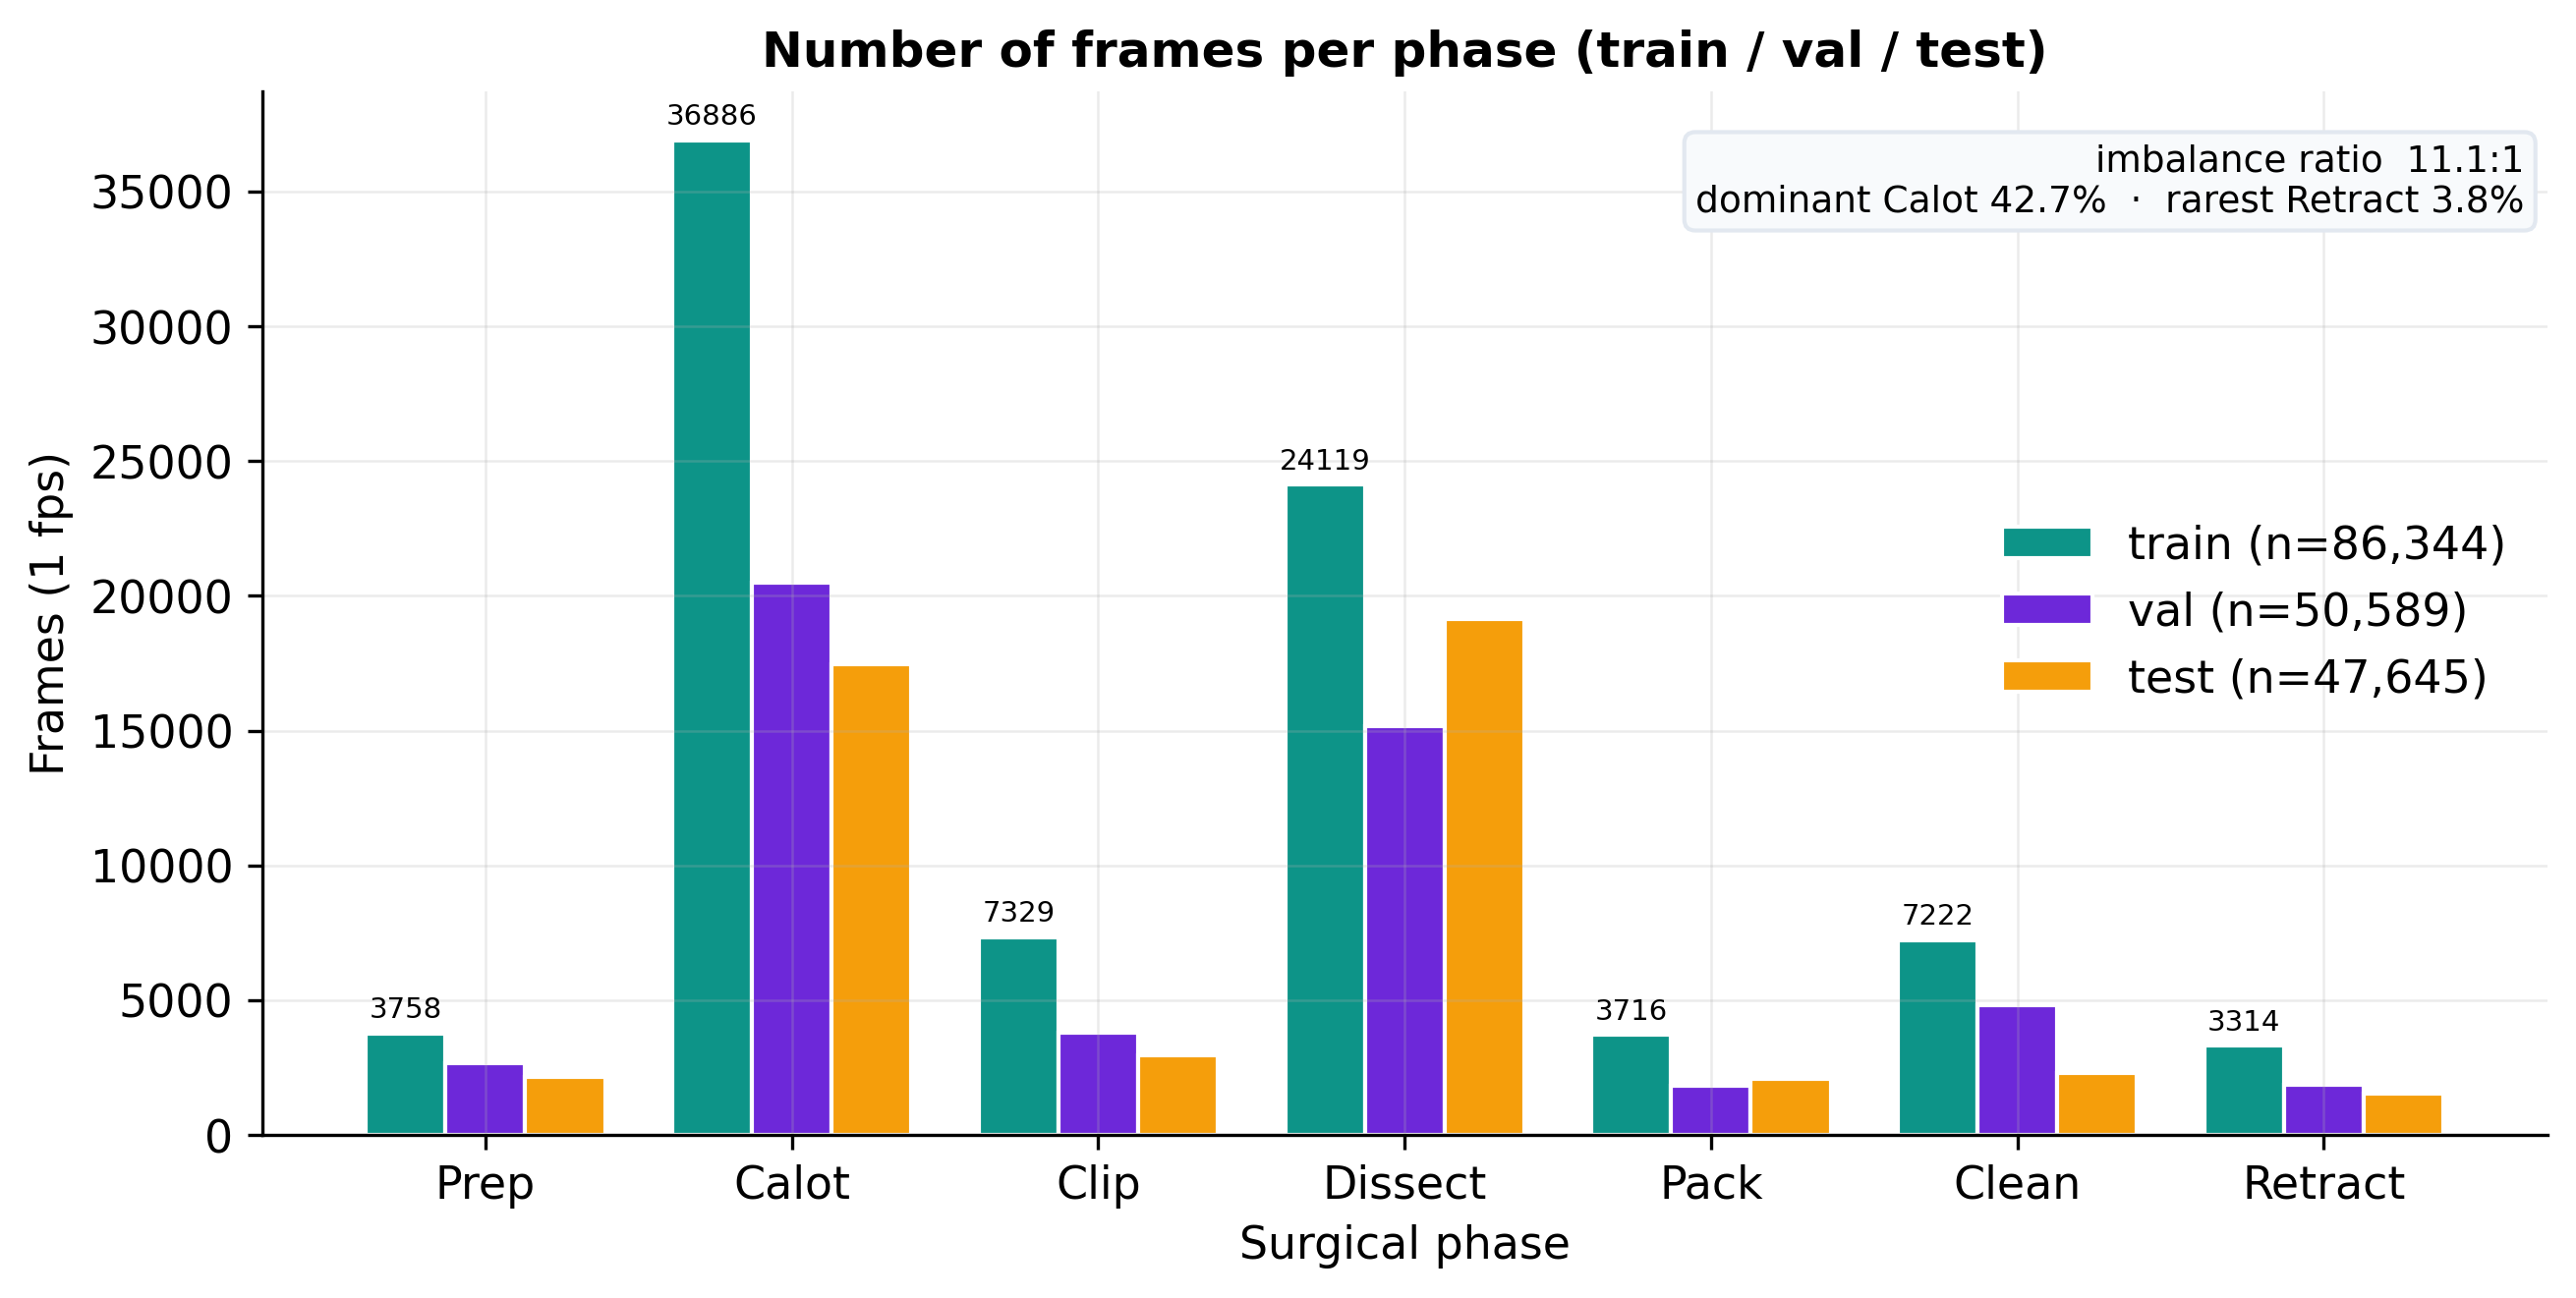
\includegraphics[width=\textwidth]{figures/class_distribution.png}
\caption{Number of frames per phase in the training, validation, and test splits. The common phases (Calot, Dissection) dominate, while the closing phases (Packaging, Retraction) are rare; the proportions are similar across splits.}
\label{fig:class_distribution}
\end{figure}

\section{Model Architectures}

Three architectures are compared, called M1, M2, and M3. All three have the same overall shape, shown in Figure~\ref{fig:transfer_learning}: a backbone turns each of the eight frames into a feature vector, a temporal model reads the sequence of eight vectors, and two small output layers predict, for each frame, the phase and which tools are present. All backbones start from ImageNet-pretrained weights~\cite{deng2009imagenet} loaded through the \texttt{timm} library~\cite{wightman2019timm}.

\begin{figure}[H]
\centering
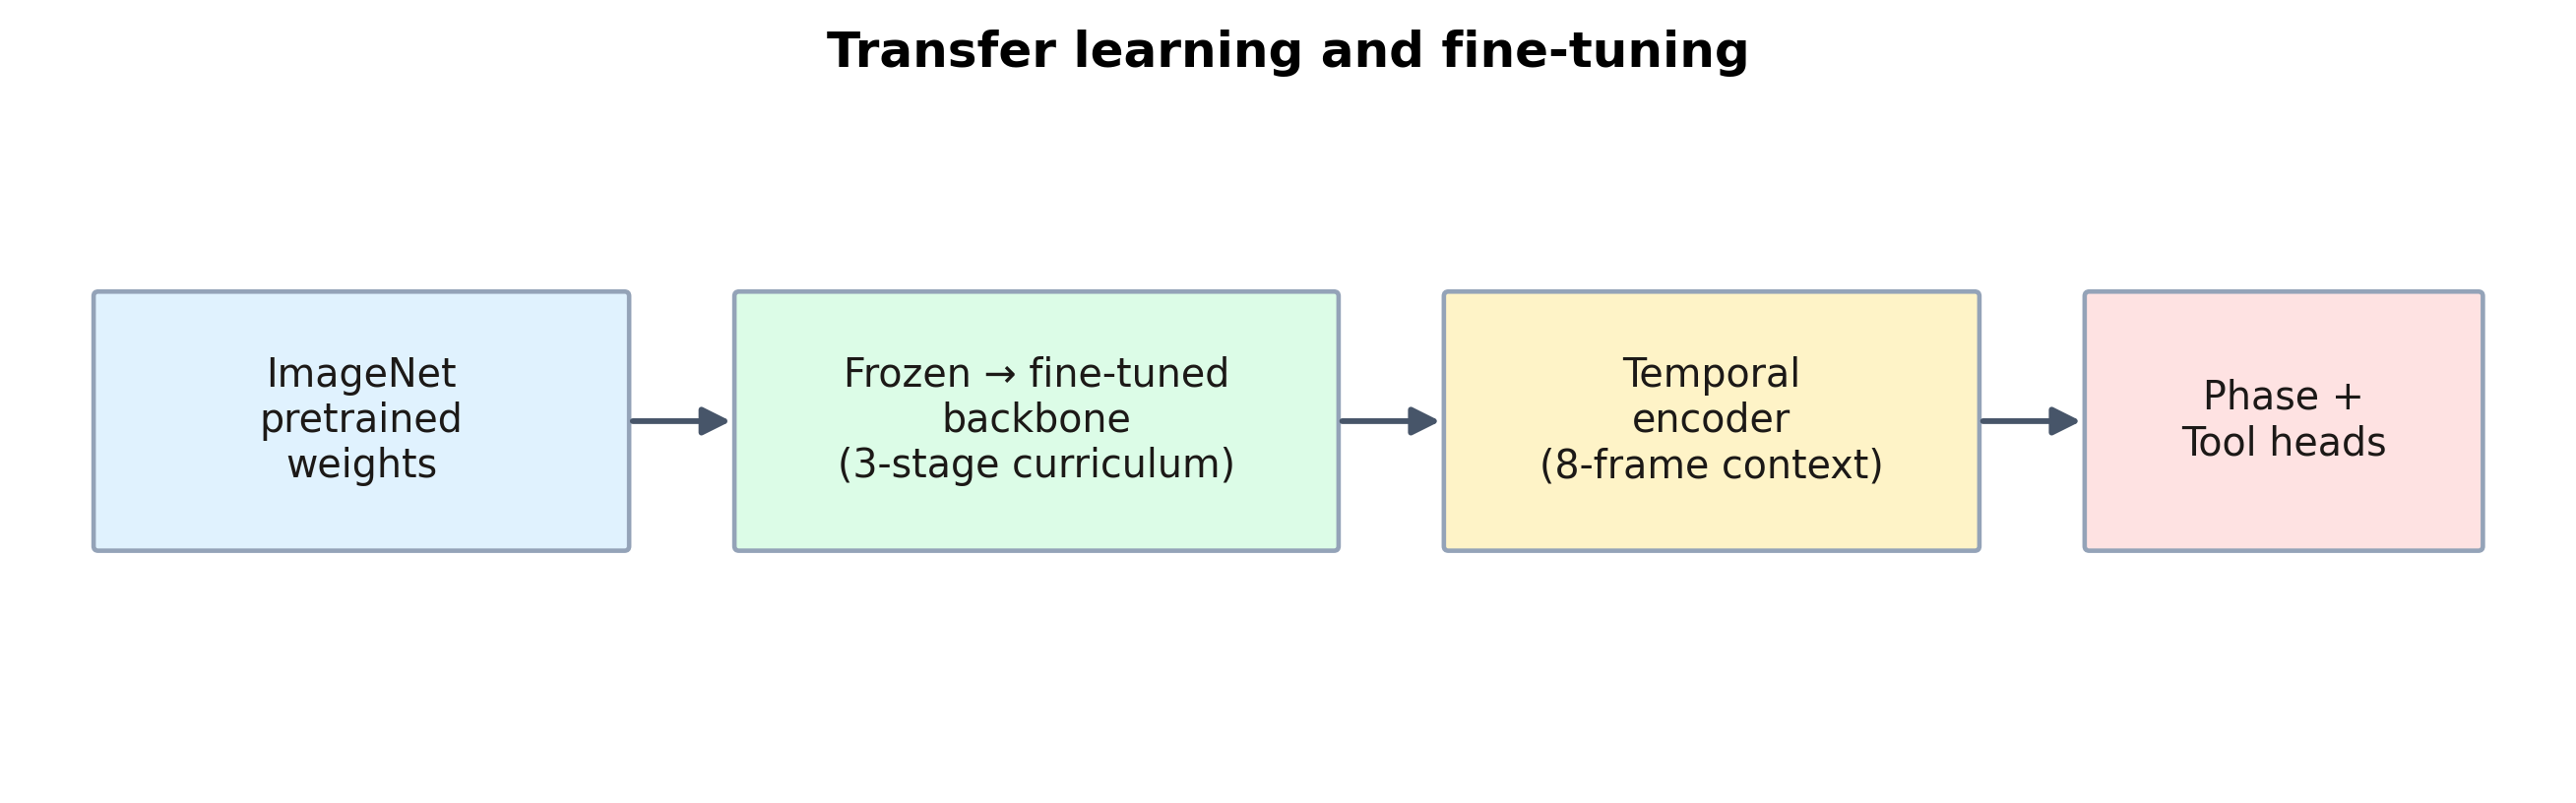
\includegraphics[width=\textwidth]{figures/transfer_learning.png}
\caption{Transfer learning and fine-tuning. The backbone starts from ImageNet weights and is fine-tuned in three stages; an eight-frame temporal model adds context; two output layers predict the phase and the tools.}
\label{fig:transfer_learning}
\end{figure}

\subsection{M1 --- ResNet-50 + Bidirectional LSTM}

The backbone is a ResNet-50~\cite{he2016deep} with ImageNet weights, giving 2048-dimensional features. The temporal model is a two-layer bidirectional LSTM with hidden size 512. Trainable parameters: 35.7~M. This follows SV-RCNet~\cite{jin2018svrcnet}.

\subsection{M2 --- EfficientNet-B3 + Temporal Convolutional Network}

The backbone is EfficientNet-B3~\cite{tan2019efficientnet} (1536-dimensional output). The temporal model is a two-stage temporal convolutional network~\cite{czempiel2020tecno} with eight dilated layers per stage and 64 filters, a smaller version of TeCNO that fits the memory budget. Trainable parameters: 11.2~M.

\subsection{M3 --- Swin-Tiny + Transformer}

The backbone is Swin Transformer-Tiny~\cite{liu2021swin} (768-dimensional output). The temporal model is a three-layer Transformer encoder~\cite{vaswani2017attention} with six heads, model size 384, and feed-forward size 768---kept small on purpose to fit the 4~GB budget. Trainable parameters: 31.6~M.

In all three models, dropout of 0.3 is applied between the temporal model and the output layers. The phase output is one linear layer giving seven scores; the tool output gives seven independent sigmoid values.

\begin{table}[H]
\centering
\caption{Summary of the three evaluated architectures.}
\label{tab:architectures}
\begin{tabular}{lllrl}
\toprule
\textbf{Model} & \textbf{Backbone} & \textbf{Temporal model} & \textbf{Params (M)} & \textbf{Family} \\
\midrule
M1 & ResNet-50      & Bidirectional LSTM  & 35.7 & CNN + RNN \\
M2 & EfficientNet-B3 & Multi-stage TCN     & 11.2 & CNN + TCN \\
M3 & Swin-Tiny      & Transformer encoder & 31.6 & ViT + Attention \\
\bottomrule
\end{tabular}
\end{table}

\section{Training Pipeline}

The training pipeline is designed around the 11:1 imbalance. It tackles the problem in four ways---class weighting, label smoothing, the extra tool task, and a staged schedule---and the ablation study (Section~\ref{sec:ablation}) measures how much each helps. Figure~\ref{fig:training_pipeline} gives an overview.

\begin{figure}[H]
\centering
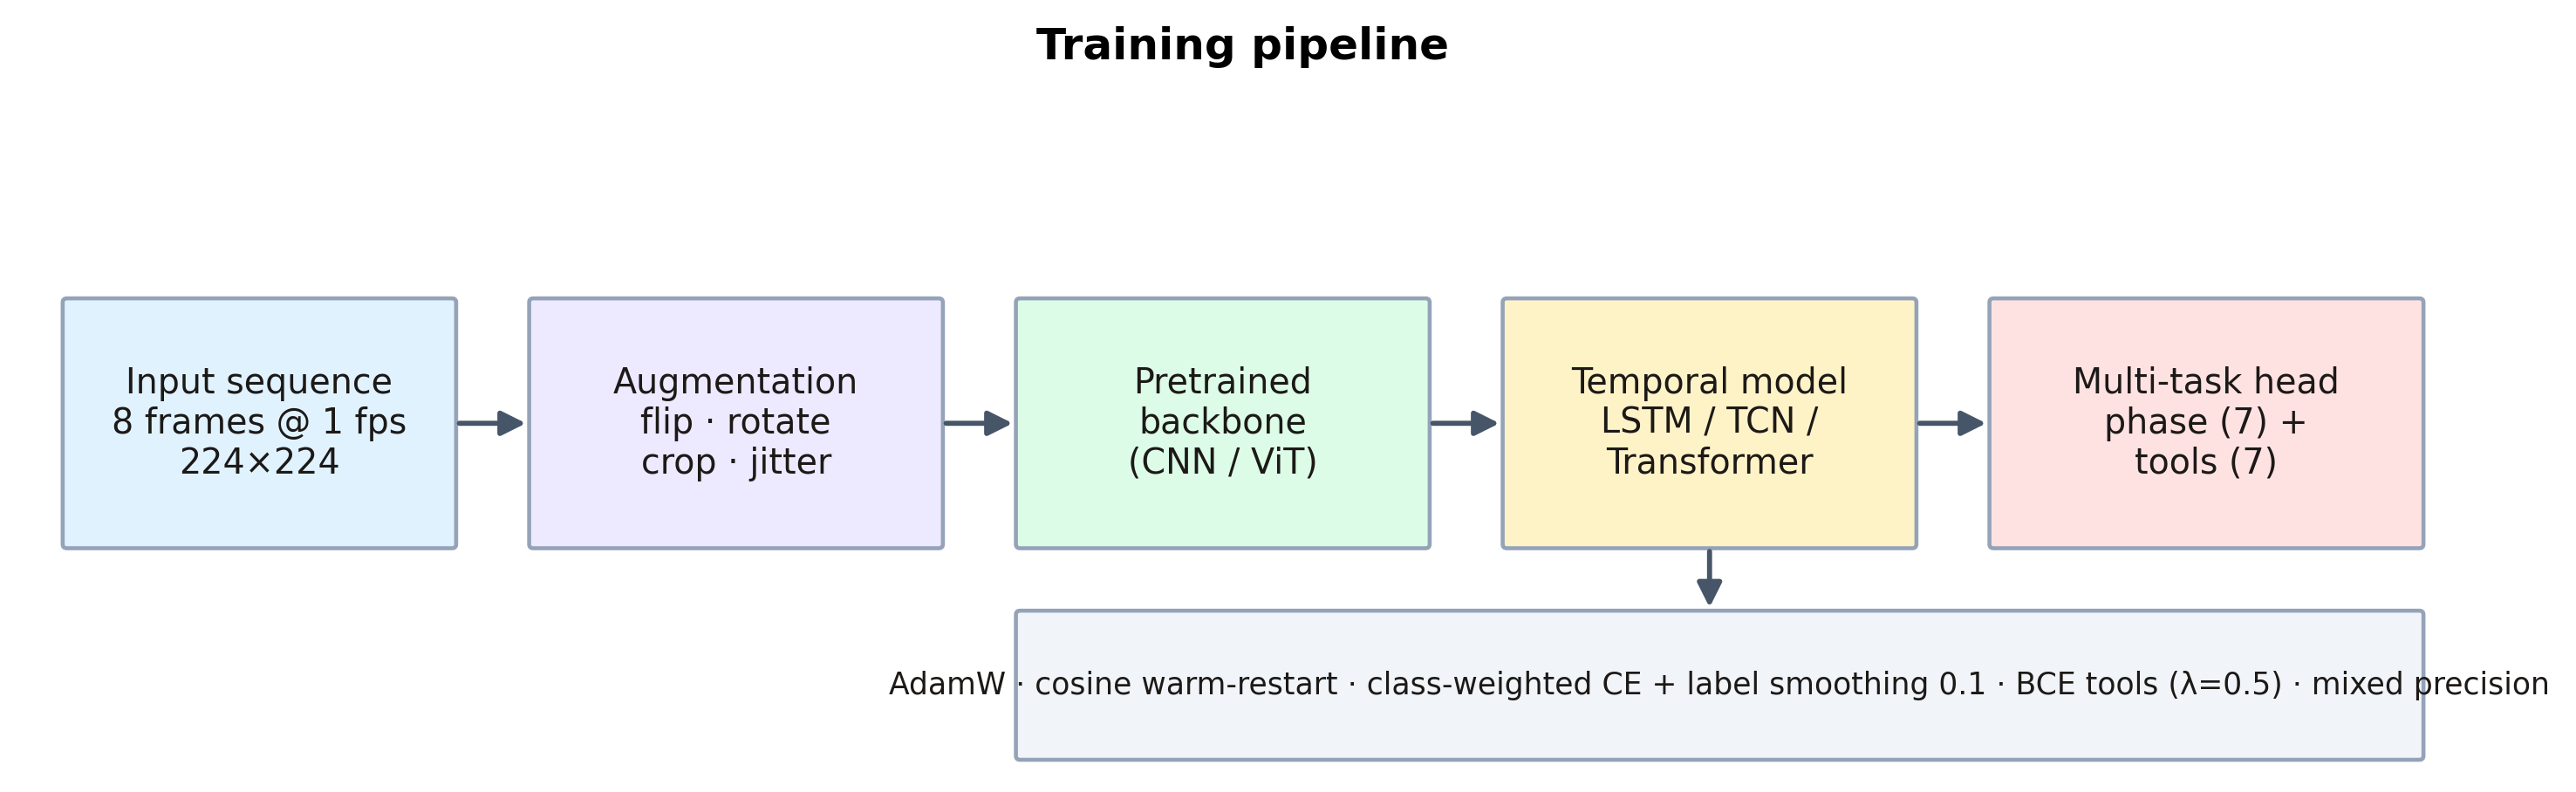
\includegraphics[width=\textwidth]{figures/training_pipeline.png}
\caption{Overview of the training pipeline. An eight-frame sequence is augmented, passed through the backbone and the temporal model, and classified by the output layers. Training uses AdamW with a cosine schedule, class-weighted cross-entropy with label smoothing for the phase, and binary cross-entropy for the tools.}
\label{fig:training_pipeline}
\end{figure}

\subsection{Loss Function}

The total loss is a weighted sum of a phase term and a tool term:
\begin{equation}
\mathcal{L} = \mathcal{L}_{\text{phase}}(z_{\text{phase}}, y_{\text{phase}}) + \lambda \cdot \mathcal{L}_{\text{tool}}(z_{\text{tool}}, y_{\text{tool}})
\label{eq:total_loss}
\end{equation}
where $\mathcal{L}_{\text{phase}}$ is class-weighted cross-entropy with label smoothing 0.1, $\mathcal{L}_{\text{tool}}$ is binary cross-entropy averaged over the seven tools, and $\lambda = 0.5$. Class weights are computed automatically as the inverse class frequency on the training split:
\begin{equation}
w_c = \frac{N}{C \cdot n_c}
\label{eq:class_weight}
\end{equation}
where $N$ is the total number of training frames, $C = 7$ is the number of phases, and $n_c$ is the number of frames in phase $c$. The weights are scaled to sum to the number of classes. This offsets the $11.1\times$ imbalance without ignoring the common phases.

\subsection{Three-Stage Schedule}

Training runs in three stages. In Stage 1 (5 epochs) the backbone is frozen and only the temporal model and output layers are trained. Stage 2 (10 epochs) continues this. In Stage 3 (10 epochs) the backbone is unfrozen and the whole network is fine-tuned, with the backbone learning rate set ten times smaller than the rest. The ablation runs use a shorter $3/6/6$ version.

\subsection{Optimisation}

The optimiser is AdamW~\cite{loshchilov2019decoupled} with a main learning rate of $1\times10^{-4}$, a backbone learning rate of $1\times10^{-5}$, weight decay of $1\times10^{-4}$, and a cosine schedule~\cite{loshchilov2017sgdr}. Mixed-precision (fp16) training~\cite{micikevicius2018mixed} keeps memory within the 4~GB budget; gradients are clipped to a maximum norm of 1.0. The batch sizes are 4 (M1), 8 (M2), and 4 (M3), the largest that fit in memory. Training stops early if validation macro-F1 does not improve for five epochs.

\subsection{Hardware and Software}

All experiments ran on one NVIDIA GeForce RTX 2050 laptop GPU (4~GB) with an Intel Core i7 CPU and 24~GB of RAM, under Windows 11, using Python 3.13, PyTorch 2.6 with CUDA 12.4, torchvision, timm, OpenCV, and scikit-learn.

\section{Evaluation Metrics}

Accuracy alone is misleading on Cholec80: a model that always predicts the two common phases scores well while ignoring the short closing phases. The following metrics are therefore reported alongside accuracy.

\begin{itemize}
    \item \textbf{Macro-F1.} The average of the seven per-phase F1 scores, giving every phase equal weight regardless of how common it is. This is the main metric for choosing models.
    \item \textbf{Per-phase precision / recall / F1.} Shown together with the confusion matrix to see where each model fails.
    \item \textbf{Edit score.} A segment-level metric that judges the quality of the predicted phase \emph{sequence} rather than each frame on its own.
    \item \textbf{Expected Calibration Error (ECE) and Negative Log-Likelihood (NLL).} Used in the calibration analysis (Section~\ref{sec:calibration}).
\end{itemize}

At test time, the predicted phase for each frame is the one with the highest score, and a median filter of length fifteen is run over each video's predictions to remove single-frame errors.

\section{Real-Time Decoding and Calibration}
\label{sec:decoding}

Besides the median filter, this thesis adds a decoder that turns the per-frame scores into a clean phase sequence using only past and present frames, so that it could run during surgery.

\subsection{Temperature Calibration}

For each model a single number $T^\star$ (the temperature) is found on the validation set by minimising the negative log-likelihood over a grid of values. Dividing the scores by $T^\star$ before the softmax tones down over-confident predictions and lowers the ECE, without changing which phase is chosen. The fitted values are 1.3 (M1), 1.1 (M2), and 1.2 (M3)---all above 1.0, which means all three models were over-confident.

\subsection{Learned Transition Table}

A transition table $A$, where $A[i, j]$ is the probability of moving from phase $i$ to phase $j$ from one second to the next, is built from the 40 training videos by counting one-step transitions at 1~fps (with a small smoothing constant). The table is strongly diagonal---the chance of staying in the same phase from one second to the next is between 0.988 and 0.999---and the off-diagonal weight sits on the next phase, matching the fixed order of cholecystectomy.

\subsection{Real-Time Decoder}

The decoder keeps a running score $\alpha_t[c]$ for each phase $c$, equal to the best total score of any path ending in phase $c$ at time $t$. At each step,
\begin{equation}
\alpha_t[c] = \log\,\text{softmax}(z_t / T^\star)[c] + \max_{c'} \big( \alpha_{t-1}[c'] + \log A[c', c] \big),
\label{eq:viterbi}
\end{equation}
and the predicted phase is the one with the highest $\alpha_t$. Each step costs only 49 operations for seven phases, so it runs much faster than real time. The calibrated scores and the transition table are added together in log space; if the scores are too sharp, the table is ignored, which is why calibration is needed for the table to help.

The decoder is compared against three baselines: raw predictions, median-15 smoothing, and an \textbf{offline} pass over the whole video that enforces the fixed phase order using future frames. The offline pass needs the full video, so it is an upper bound, not a method that could run live.

\section{Ablation and Ensemble Design}

Four ablations each change one thing relative to the M1 baseline, to see what that one thing is worth: \textbf{A1} removes the tool-detection task (phase only); \textbf{A2} removes class weighting (plain cross-entropy); \textbf{A3} doubles the sequence to sixteen frames and halves the batch size; and \textbf{A4} turns off the median filter at test time.

Three ways of combining the three models are tested: \textbf{simple averaging} of their predictions, \textbf{averaging weighted by validation F1}, and \textbf{majority voting} over their per-frame choices. All three pass through the same median filter before evaluation. The weighted average is
\begin{equation}
\hat{y} = \arg\max_c \sum_{m=1}^{M} \omega_m \, p_m(c \mid x),
\label{eq:ensemble}
\end{equation}
where $M = 3$ is the number of models, $p_m(c \mid x)$ is the probability model $m$ gives to phase $c$, and the weight $\omega_m$ is proportional to model $m$'s validation macro-F1.
